\documentclass[
    11pt,
    spanish,
	a4paper
]{article}
\usepackage[utf8]{inputenc}
\usepackage[spanish]{babel}
\usepackage{graphicx}
\usepackage{authoraftertitle}
\usepackage{float}
\usepackage{caption}
\captionsetup[table]{labelformat=empty}
\usepackage{listings}


\def\doctype{PRUEBAS DE ACEPTACIÓN Y SISTEMA}
\title{Evaluador de microcontroladores para misiones espaciales}
\author{Gonzalo Nahuel Vaca}

\begin{document}

\makeatletter
\begin{titlepage}
	\begin{center}
		\vspace*{1cm}
		
		\Huge
		\textbf{\doctype}
		
		\vspace{0.5cm}
		\LARGE
		\@title
		
		\vspace{1.5cm}
		
		\textbf{\@author}

		\vspace{3.5cm}

		
\includegraphics[width=0.8\textwidth]{img/logoFIUBA.pdf}
		
		\vfill
		Facultad de Ingeniería\\
		Universidad de Buenos Aires\\
		Argentina\\
		\today
	\end{center}
\end{titlepage}
\makeatother
\newpage

\section{Introducción}
\label{sec:introduccion}

Este documento tiene el objetivo de planificar los ensayos de nivel de sistema y de nivel de aceptación para un módulo del proyecto ``\MyTitle''.

El módulo seleccionado es el ``Validador de periférico SPI'', quién deberá determinar si el integrado aún cuenta con un sistema SPI funcional.

El código del módulo es el siguiente:

\begin{lstlisting}[language=C]
bool validate_SPI()
{
    uint8_t spi_write[5] = {1, 2, 3, 4, 5};
    uint8_t spi_read[5] = {6, 7, 8, 9, 10};
    uint8_t status = NORMAL;
    SPI0_WriteRead(&spi_write[0], 5, &spi_read[0], 5);
    for(uint8_t i = 0; i < 5; ++i)
    {
        if(spi_write[i] != spi_read[i])
        {
            status = ERROR;
            break;
        }
    }
    return status;
}
\end{lstlisting}

\section{Pruebas a nivel sistemas}
\label{sec:lvlsistema}

Las pruebas de este nivel se realizan considerando un conocimiento pleno sobre el código fuente.
Por este motivo se realizarán bajo el esquema de \emph{Elementary Comparison Test}.

\begin{table}[H]
	\centering
	\begin{tabular}{c|cc}
        C1 \& C2 \& C3 \& C4 \& C5 & NORMAL & ERROR \\ \hline
        1.1.1.1.1                  & +      &       \\
        1.1.1.1.0                  &        & +     \\
        1.1.1.0.1                  &        & +     \\
        1.1.0.1.1                  &        & +     \\
        1.0.1.1.1                  &        & +     \\
        0.1.1.1.1                  &        & +     \\
	\end{tabular}
\end{table}

Para realizar estas pruebas se necesitará realizar un \emph{mock} de la función de escritura y lectura del periférico SPI.

\section{Pruebas a nivel aceptación}
\label{sec:lvlaceptacion}

Las pruebas de este nivel se realizan considerando al módulo como una caja negra.
Por este motivo se realizarán bajo el esquema de \emph{Classification-tree Method}.
En la figura \ref{fig:ctm} se puede observar el diagrama con los dos casos de prueba.
El caso ``1'' consiste en dejar conectado del \emph{loopback} del periférico, mientras que el caso ``2'' se realiza desconectado la conexión entre la entrada y salida del módulo SPI.

\begin{figure}[h!]
	\centering
	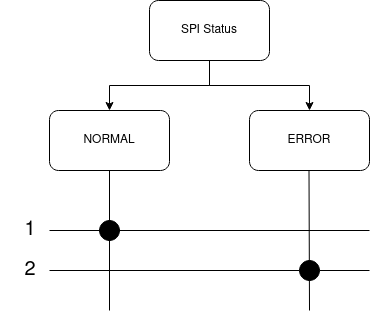
\includegraphics[width=0.7\textwidth]{./img/ctm.png}
    \caption{Diagrama \emph{Classification-tree Method}.}
	\label{fig:ctm}
\end{figure}

La pruebas se realizarancon el siguiente script de \emph{Python}:

\begin{lstlisting}[language=Python]
from serial import Serial
import signal, os

def handler(signum, frame):
    print("")
    print("Terminal ended by user")
    exit()

def main():
    with Serial('/dev/ttyACM0', 9600, timeout=1) as s:
        while True:
            x = s.read()
            if x == b'R':
                f = ord(s.read())
                c = int.from_bytes(s.read(4), 'little')
                print("FLAGS:", f, "COUNTER:", c, end='\r')

if __name__ == "__main__":
    signal.signal(signal.SIGINT, handler)
    main()
\end{lstlisting}

\end{document}
